% sos2cayley gf_aa.sos --rename a=a,!a=b
% Generated by sosl.sos.viz. Every visual choice is in the \tikzset below:
% edit a style to restyle, edit a coordinate to move a node.
\documentclass[tikz,border=4pt]{standalone}
\usetikzlibrary{arrows.meta,shapes.misc}
\begin{document}
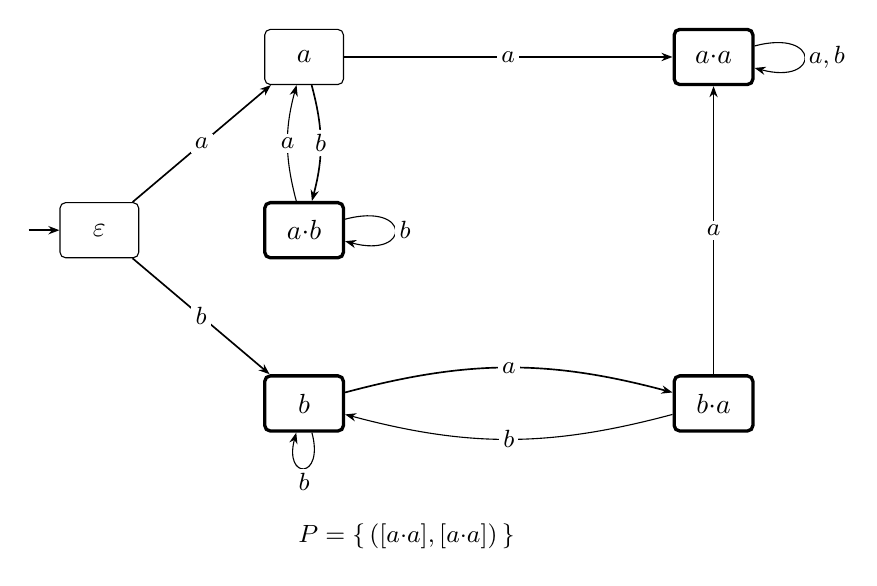
\begin{tikzpicture}[
  class/.style     = {draw, thin, rounded corners=2pt, inner sep=3pt,
                      minimum width=10mm, minimum height=7mm},
  root/.style      = {},          % the root needs no ink: the init stub says it
  idem/.style      = {very thick},
  init/.style      = {semithick, -{Stealth[length=4pt,width=3pt]}},
  tree/.style      = {semithick, -{Stealth[length=4pt,width=3pt]}},
  nontree/.style   = {thin, -{Stealth[length=4pt,width=3pt]}},
  lbl/.style       = {font=\small, inner sep=1.5pt, fill=white},
  pairs/.style     = {anchor=north, font=\small},
]

  % grid: x horizontal, y down from the top left; cols 0,1,3 / rows 0,1,2.
  \node[class,root] (eps) at (0.0,-2.2) {$\varepsilon$};        % 0,1
  \node[class] (a) at (2.6,0.0) {$a$};                          % 1,0
  \node[class,idem] (ab) at (2.6,-2.2) {$a{\cdot}b$};           % 1,1
  \node[class,idem] (b) at (2.6,-4.4) {$b$};                    % 1,2
  \node[class,idem] (aa) at (7.8,0.0) {$a{\cdot}a$};            % 3,0
  \node[class,idem] (ba) at (7.8,-4.4) {$b{\cdot}a$};           % 3,2

  % the root is the adjoined identity: a source, marked like an initial state
  \draw[init] (-0.9,-2.2) -- (eps);

  \draw[tree] (eps) to node[lbl] {$a$} (a);
  \draw[tree] (eps) to node[lbl] {$b$} (b);
  \draw[tree] (a) to node[lbl] {$a$} (aa);
  \draw[tree] (a) to[bend left=15] node[lbl] {$b$} (ab);
  \draw[tree] (b) to[bend left=15] node[lbl] {$a$} (ba);
  \draw[nontree] (b) to[loop below] node[lbl] {$b$} (b);
  \draw[nontree] (aa) to[loop right] node[lbl] {$a,b$} (aa);
  \draw[nontree] (ab) to[bend left=15] node[lbl] {$a$} (a);
  \draw[nontree] (ab) to[loop right] node[lbl] {$b$} (ab);
  \draw[nontree] (ba) to node[lbl] {$a$} (aa);
  \draw[nontree] (ba) to[bend left=15] node[lbl] {$b$} (b);

  \node[pairs] at (3.9,-5.8) {$P = \{\, ([a{\cdot}a],[a{\cdot}a]) \,\}$};
\end{tikzpicture}
\end{document}
